%%Tema para beamer "Imunam", versión 1.0
%%Desarrollado por Geri Morales (gerino.morales@im.unam.mx)
%%Imate Cuernavaca, UNAM. Agosto 2014.

\documentclass{beamer}
\usepackage[utf8]{inputenc}
\usepackage[T1]{fontenc} 
\usepackage[spanish]{babel} 
\usepackage{multicol}
\setlength{\columnsep}{1cm}

%%Se define el "environment" teorema
\newtheorem{frase}{Frase}


%%Tema de beamer "Imunam"
\usetheme[cuernavaca]{Imunam} 
%\usetheme{Imunam} 
%%Si se omite "[cuernavaca]" en éste comando, el logotipo se imprime sin la 
%%leyenda "Unidad Cuernavaca" en la parte inferior.


\title{La incertidumbre de la ciencia}
\author{Oscar Rodriguez Arroyo 
	      \texttt{oscar.rodar@gmail.com}} %Dirección de correo electrónico (opcional, cuidado con la llave de cierre)
	      
\date{Basada en una conferencia de Richard P. Feynman - 19/01/2016}

\begin{document}

\begin{frame}

  \titlepage %Necesario para generar la portada
  
\end{frame}

%%La siguiente diapositiva es opcional, si se quiere la tabla de contenidos
%%Se sebe compilar dos veces el documento para que funcione
%--------------------------------------------------------------------------
%\begin{frame}
%\tableofcontents %Imprime la tabla de contenido
%\end{frame}
%--------------------------------------------------------------------------

%--------------------------Slide Agenda
%\section{Agenda} %%Título de la sección (Opcional)
\begin{frame}
  \frametitle{Agenda}

  \begin{itemize}
    \item Hipótesis
    \item Introducción - Richard Feynman  
    \item Aspectos de la Ciencia
    \item Hipótesis e Ideas
    \item La Incertidumbre 
    \item Gracias  
    
  \end{itemize}
 
\end{frame}

%--------------------------Slide Motivación

\begin{frame}
    \frametitle{Hipótesis}
    \begin{frase}
        Lo más maravilloso de la ciencia es que está viva
    \end{frase}
    
\end{frame}

%--------------------------Slide Intro 

\begin{frame}
  \frametitle{Richard Phillips Feynman}
  \framesubtitle{¿Quién fue?}
    \begin{multicols}{2}
    \begin{figure}[htp]
        \centering
        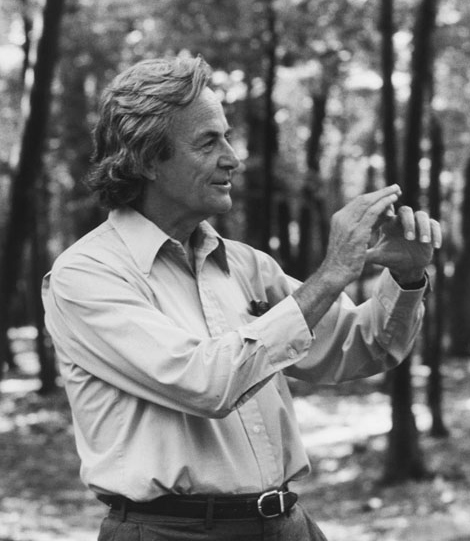
\includegraphics[width=3cm]{images/RF}
        \caption{Richard Feynman}
        %% «RichardFeynman-PaineMansionWoods1984 copyrightTamikoThiel bw» de Copyright Tamiko Thiel 1984 - OTRS communication from photographer. Disponible bajo la licencia CC BY-SA 3.0 vía Wikimedia Commons - https://commons.wikimedia.org/wiki/File:RichardFeynman-PaineMansionWoods1984_copyrightTamikoThiel_bw.jpg#/media/File:RichardFeynman-PaineMansionWoods1984_copyrightTamikoThiel_bw.jpg
    \end{figure}

  \begin{itemize}
    \item Físico Teórico
    \item Reconocimientos
    \item Proyecto Manhattan 
  \end{itemize}
  \end{multicols}
 
\end{frame}

%--------------------------Ciencia segun Feynman 

\begin{frame}{Ciencia}
    \frametitle{Ciencia}
    \framesubtitle{¿Qué es?}
    
    \begin{multicols}{2}
      
      \begin{itemize}
        \item Descubrimiento
        \item Cuerpo de conocimiento
        \item Aplicacaciones de la ciencia (Tecnología)
      \end{itemize}
      
      \begin{figure}[htp]
        \centering
        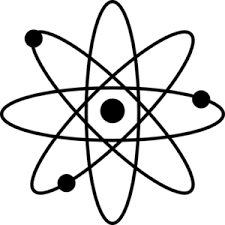
\includegraphics[width=3cm]{images/atomo}
        \caption{Átomo}
    \end{figure}
    \end{multicols}
\end{frame}

%--------------------------Slide Tecnología
\begin{frame}{Tecnología}
\frametitle{Tecnología}
\begin{itemize}
    \item Característica Obvia
    \item Ejemplos
    \item "Todo gran poder conlleva una gran responsabilidad"
    \item Problemas relacionados
\end{itemize}
    
\end{frame}

%--------------------------Slide Cuerpo de conocimiento 
\begin{frame}{Cuerpo de conocimiento}
\frametitle{Cuerpo de conocimiento}
 \begin{multicols}{2}
\begin{itemize}
    \item Importancia 
    \item Razón de descubrir 
    \item La ignorancia
    \item La imaginación 
    \item Seres vivos
\end{itemize}


\begin{figure}[htp]
        \centering
        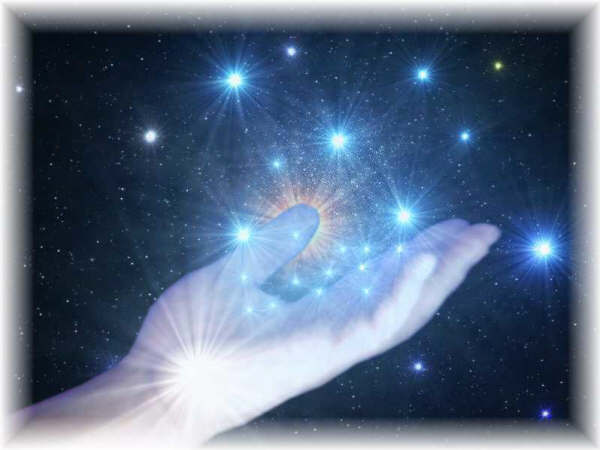
\includegraphics[width=3cm]{images/dust}
        \caption{"Polvo de estrellas"}
    \end{figure}

\end{multicols}
\end{frame}

%--------------------------Slide Métodos científicos

\begin{frame}{Ciencia como método}
\frametitle{Ciencia como Método}
\begin{multicols}{2}

\begin{itemize}
    \item ¿Quien juzga? 
    \item La excepción 
    \item Limitaciones y preguntas
    \item Características
    \item Resultados
\end{itemize}

\begin{figure}[htp]
        \centering
        
\includegraphics[width=3cm]{images/observacion}
        \caption{Método Científico}
    \end{figure}

\end{multicols}
\end{frame}

%--------------------------Diapositiva Reglas 
\begin{frame}{Hipótesis e Ideas}
    \frametitle{Hipótesis e Ideas}
    
    \begin{figure}[htp]
        \centering
        
\includegraphics[width=3cm]{images/idea}
        \caption{Hipótesis}
    \end{figure}
    
\end{frame}

%--------------------------Diapositiva de Ideas 
\begin{frame}{La Incertidumbre}
    \frametitle{La Incertidumbre}
    
        \begin{figure}[htp]
        \centering
        
\includegraphics[width=3cm]{images/duda}
        \caption{Incertidumbre}
    \end{figure}
    
\end{frame}

%--------------------------Diapositiva de Gracias

\begin{frame}
    \frametitle{Gracias}
    \begin{frase}
        Lo más maravilloso de la ciencia es que está viva - Richard Feynman
    \end{frase}
    
\end{frame}


\end{document}